\section{A First Naïve Approach Using Partial Orders}

\begin{figure}
\centering
\begin{subfigure}[b]{0.49\textwidth}
\centering
	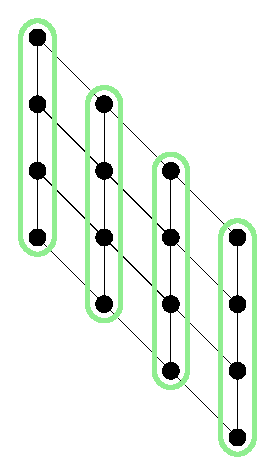
\includegraphics[width=0.4\textwidth]{fig/x+y/poset/chains}
	\caption{Balanced selection of disjoint chains in \XY.}
	\label{fig:xy:poset:chains}
\end{subfigure}
\begin{subfigure}[b]{0.49\textwidth}
\centering
	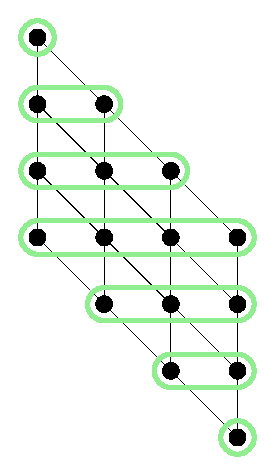
\includegraphics[width=0.4\textwidth]{fig/x+y/poset/antichains}
	\caption{Maximal antichains in \XY.}
	\label{fig:xy:poset:antichains}
\end{subfigure}
\end{figure}

\begin{figure}
\centering
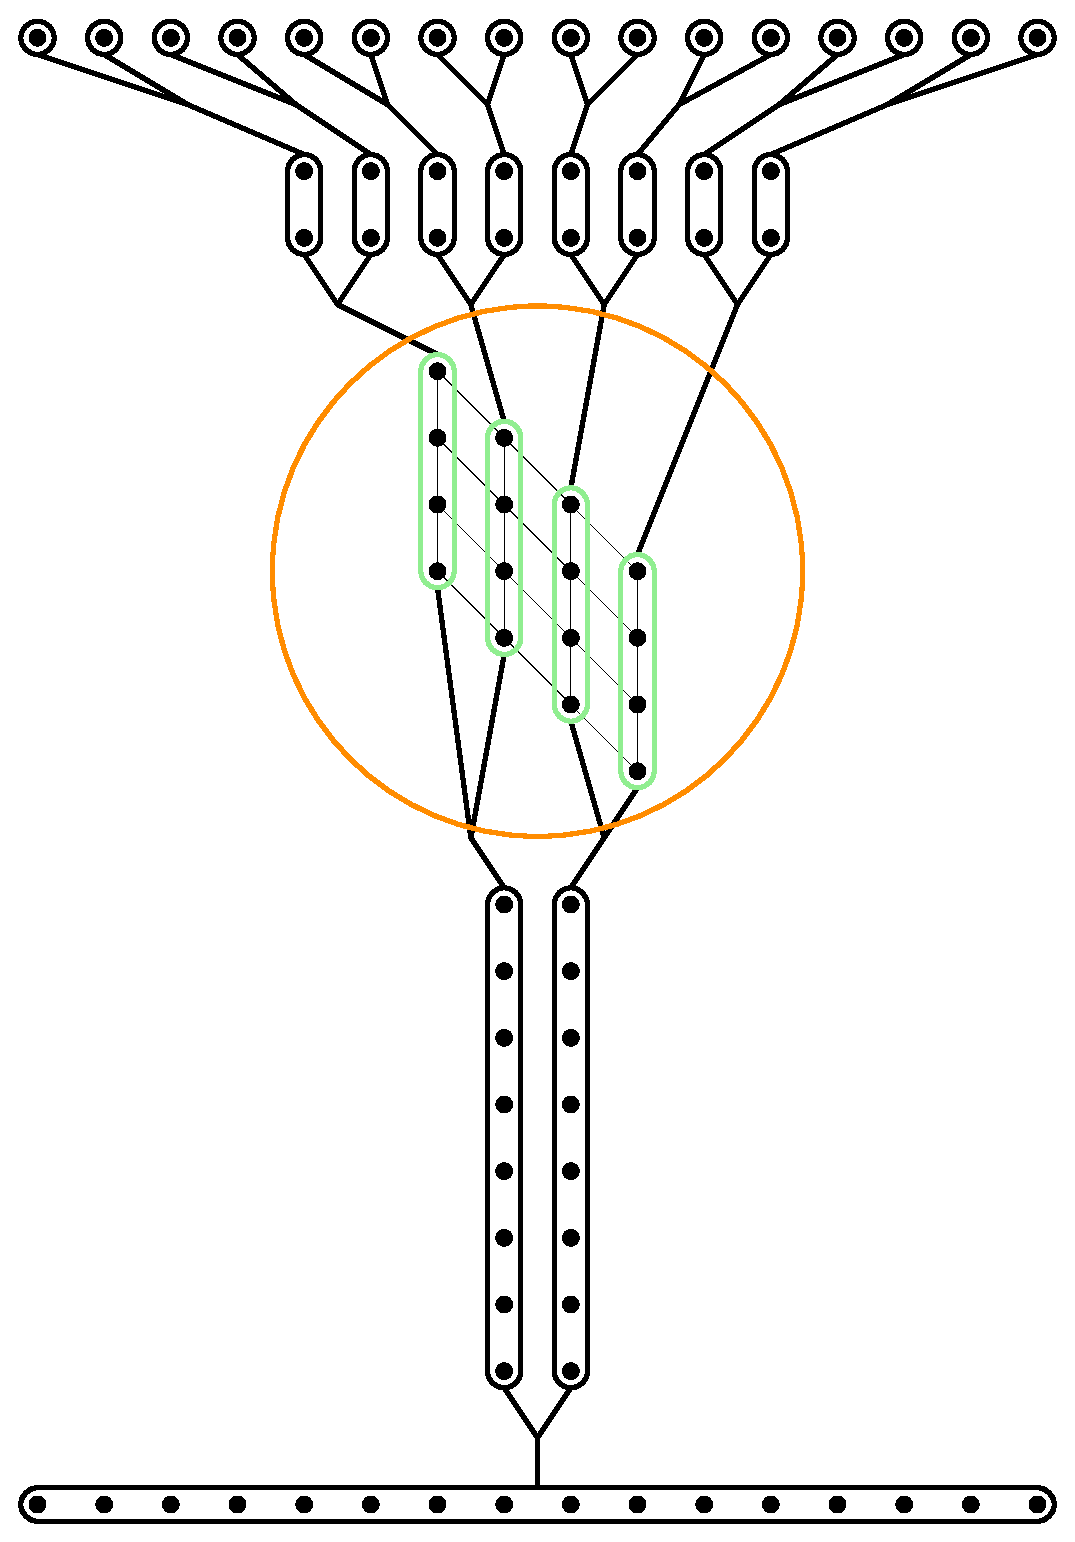
\includegraphics[width=0.5\textwidth,angle=90]{fig/x+y/poset/mergexy}
\caption{Resolution of the mergesort algorithm with the part
corresponding to the starting point of a sort \XY problem highlighted.}
\label{fig:xy:poset:mergexy}
\end{figure}

In this first, naïve, attempt we will use the partial order structure on the
elements in \XY to reduce by a factor of $2$ the number of comparisons required
to sort \XY compared to the execution of a simple mergesort algorithm.

In \ref{tree:open:xy} we saw \ref{fig:open:xy} which shows us all the order
relations between elements of \XY. Now, we will see that chains and antichains
in \XY obey to a regular pattern. To illustrate this, we take the $4 \times 4$
\XY problem. We highlight a possible selection of disjoint chains in
\ref{fig:xy:poset:chains} and the set of maximal antichains in
\ref{fig:xy:poset:antichains}.

Now we will solve this problem in a strictly faster way than sorting all
of its elements, by taking advantage of some of the information we already have.

First, note that sorting $X + Y$ without information using the merge sort
algorithm would use $2 n^2 \log n$ comparisons. We will show that it is
possible to sort $X + Y$ with half the comparisons.

The merge sort algorithm has this particularity that at the end of every step
of the recursion we are left with several total orders on disjoint subsets of
the set to sort. To illustrate, if we organise steps in stages we obtain what
is shown in \ref{fig:xy:poset:mergexy}.

What is highlighted in \ref{fig:xy:poset:mergexy} is a subset of the
information we have when knowing the structure of \XY, \ie the chains of
\ref{fig:xy:poset:chains}. It means that this specific stage we
highlighted can be attained without any comparison if the set to sort is \XY
and that we know its structure.

Remember that in merge sort there are $\log N$ stages. At stage $i$ we have
built $2^{i}$ total orders on disjoint subsets of size $2^{\log N - i}$. Since
the stage represented in \ref{fig:xy:poset:mergexy} shows $n$ total orders on
disjoint subsets of size $n$, and that the total number of elements in $X+Y$ is
$N = n^2$ we can conclude that \ref{fig:xy:poset:mergexy} shows us step
$\sfrac{1}{2} \log N$. In merge sort, at each stage of the recursion we do at
most N comparisons hence we only have half of the comparisons left to do in
order to complete the execution of the algorithm.
